%----------------------------------------------------------------------------------------
%	PROBLEM 6
%----------------------------------------------------------------------------------------
%----------------------------------------------------------------------------------------
\section{Problem VI}
Consider a light ray entering two adjacent planes of glass on a table. At any meeting surface (between the two planes of glass, or between the top glass and the air) the light may either reflect (bounce) or continue straight through (refract). In the example below, the light ray bounces 7 times before it leaves the glass plane. The light always reflects between the bottom glass and the table. How many different paths can a light ray take if it bounces $n$ times before it leaves the top glass plane? Give a recurrence relation to answer this question.\\\\
\textbf{Solution:} \\
According to the Figure of problem, we can notice that for any $n$ is even, $F(n) = 0$.\\
If $n$ is an odd, we will have following 5 basic paths below for the last two reflections before it leaves table:\\
\begin{figure}[h]
	\centering
	\subfloat[Subfigure 1 list of figures text][Path case 1]{
		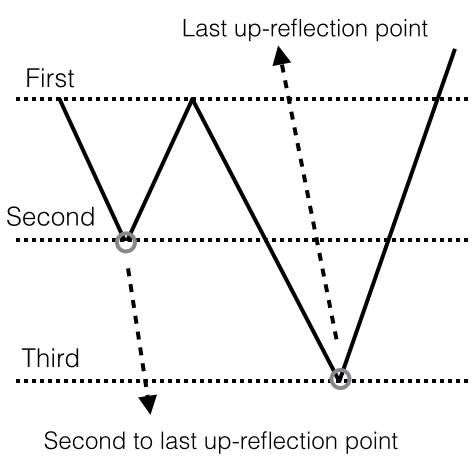
\includegraphics[width=0.2\textwidth]{path1}
		\label{fig:p6subfig1}}
	\subfloat[Subfigure 2 list of figures text][Path case 2]{
		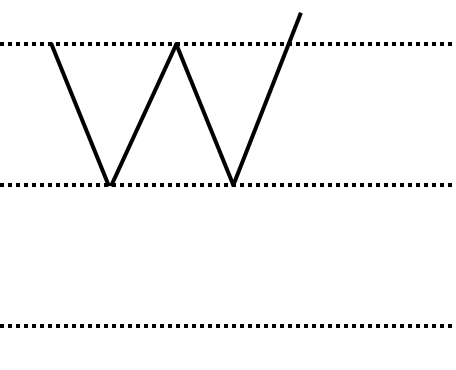
\includegraphics[width=0.2\textwidth]{path2}
		\label{fig:p6subfig2}}\\
	\subfloat[Subfigure 3 list of figures text][Path case 3]{
		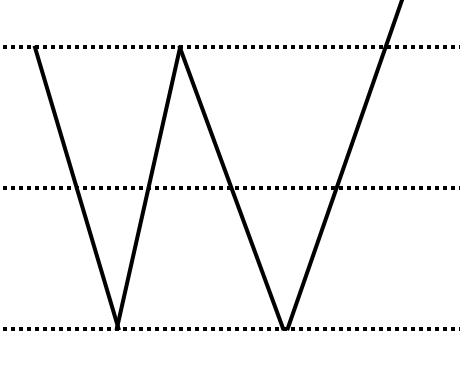
\includegraphics[width=0.2\textwidth]{path3}
		\label{fig:p6subfig3}}
	\subfloat[Subfigure 4 list of figures text][Path case 4]{
		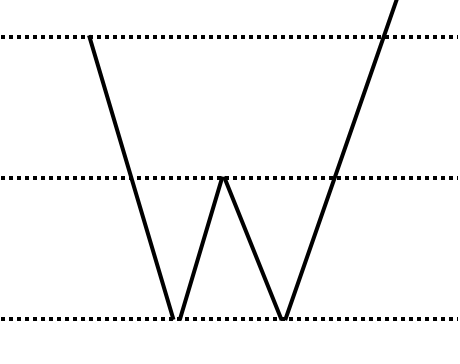
\includegraphics[width=0.2\textwidth]{path4}
		\label{fig:p6subfig4}}
	\subfloat[Subfigure 5 list of figures text][Path case 5]{
		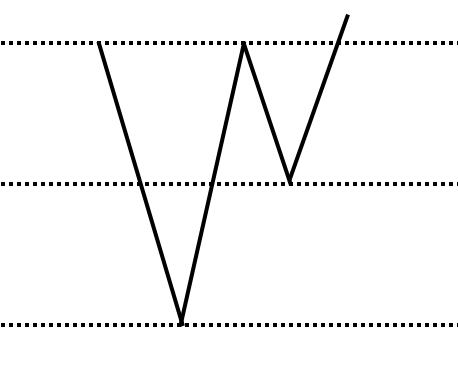
\includegraphics[width=0.2\textwidth]{path5}
		\label{fig:p6subfig5}}
	\caption{5 basic paths for the last two reflections}
	\label{fig:p6fig}	
\end{figure}\\
As shown in Figure \ref{fig:p6fig}, we can note that if the second to last up-reflection point is on the second level from the top, there are two kinds possible paths to leave table as shown in Figure \ref{fig:p6subfig1} and Figure \ref{fig:p6subfig2}. We can also notice that if the second to last up-reflection point is on the second level from top, the last up-reflection point will have $\frac{1}{2}$ possiblity to be on the second level from top as shown in Figure \ref{fig:p6subfig1} and $\frac{1}{2}$ possiblity to be on the third level from top as shown in Figure \ref{fig:p6subfig2}. However, if the second to last up-reflection point is on the third level from top, there are three kinds of possible paths to leave table as shown in Figure \ref{fig:p6subfig3}, Figure \ref{fig:p6subfig4} and Figure \ref{fig:p6subfig5}. Similarly, we could note that if the second to last up-reflection point is on the third level from top, the last up-reflection point will have $\frac{1}{3}$ possiblity to be on the second level from top as shown in Figure \ref{fig:p6subfig5} and $\frac{2}{3}$ possiblity to be on the third level from top as shown in Figure \ref{fig:p6subfig3} as well as Figure \ref{fig:p6subfig4}.\\\\

Based on the discussion above, we could analysis possible paths for $F(n)$. To get the recurrence relation of $F(n)$, we need to analyze $F(n - 2)$ and $F(n - 4)$. \\\\
we could assume that there are $p_1$ numbers of paths in $F(n - 4)$ whose last up-reflection point is on the third level from top and $p_2$ numbers of paths in $F(n - 4)$ whose last up-reflection point is on the second level from top. Thus, we have:
$$ F(n - 4) = p_1 + p_2 $$
Also, according to the disscussion and Figure \ref{fig:p6fig} above, we have:
$$ F(n - 2) = 3p_1 + 2p_2 $$
\begin{align*}
F(n) &= 3[(3p_1)\cdot \frac{2}{3} + (2p_2)\cdot \frac{1}{2}] + [(3p_1)\cdot \frac{1}{3} + (2p_2)\cdot \frac{1}{2}]\\
&= 8p_1 + 5p_2
\end{align*}
Based one this three equations, we can get $p_1 = F(n - 2) - 2F(n - 4)$, $p_2 = 3F(n - 4) - F(n - 2)$.
Thus, we have
\begin{align*}
F(n) = 
\begin{cases}
0 & n $ is even$\\
3F(n - 2) - F(n - 4) & n $ is odd$
\end{cases}
\end{align*}


